% Renders the paper's three figures from the data files in this folder, which
% scripts/08_make_figures.py writes. Build from the repository root:
%
%   xelatex -output-directory=figures figures/render_figures.tex
%
% The text width is the paper's (122 mm, Springer proceedings layout), so the
% figures come out at the size they have in the paper.
\documentclass[10pt]{article}
\usepackage[a4paper, textwidth=122mm, top=25mm]{geometry}
\usepackage{newtxtext,newtxmath}  % Times, as in the paper
\usepackage{xcolor}
\usepackage{pgfplots}
\usepackage{pgfplotstable}
\usepackage{tikz}
\usetikzlibrary{positioning,arrows.meta,fit,backgrounds}
\pgfplotsset{compat=1.18}
\definecolor{accent}{HTML}{1F4E79}
\definecolor{muted}{HTML}{8C8C8C}
\pagestyle{empty}
\setlength{\parindent}{0pt}

\begin{document}

\begin{center}
% Figure 1: how the benchmark is built (a) and what the task is (b).
%
% The audience at this venue is not an NLP audience, so this figure carries the
% task definition on its own. Row (a) was added in the revision, when
% a reviewer asked for more figures: it shows where the 1,000 test sentences
% come from and the held-out set used to check the trained baseline, with the
% counts the text quotes (script 01 for the first four boxes, script 16 for the
% last). Row (b) is the submitted figure unchanged in content.
%
% Nodes are placed at explicit coordinates rather than with `right=of`.
% Chaining off a midpoint coordinate between two boxes measures the gap from
% that coordinate, not from the boxes' edges, which once overlapped the model
% box on top of the inputs.
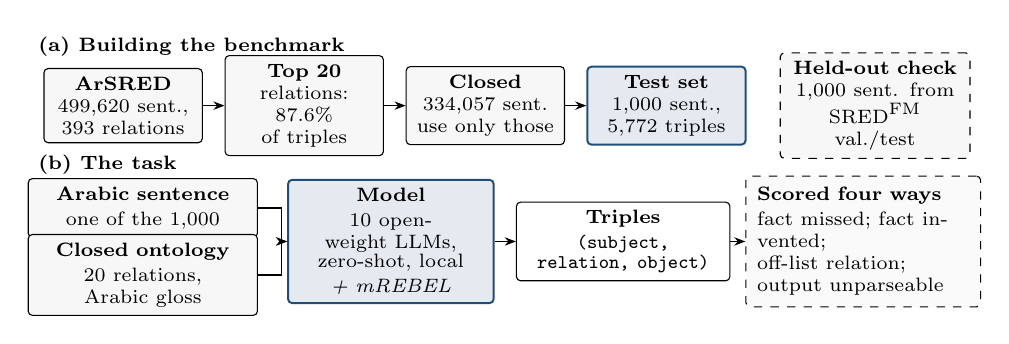
\begin{tikzpicture}[
  font=\scriptsize,
  box/.style={draw, rounded corners=1.5pt, align=center, inner sep=3pt,
              minimum height=9mm, line width=0.4pt},
  input/.style={box, fill=black!3, text width=27mm},
  stage/.style={box, fill=black!3, text width=22mm},
  model/.style={box, fill=accent!12, draw=accent, line width=0.7pt,
                text width=24mm},
  outbox/.style={box, fill=white, text width=25mm},
  scored/.style={draw, dashed, rounded corners=1.5pt, line width=0.4pt,
                 fill=black!2, align=left, inner sep=4pt, text width=27mm},
  flow/.style={-{Stealth[length=4pt]}, line width=0.5pt},
  tag/.style={font=\scriptsize\bfseries, anchor=west},
]

% --- (a) building the benchmark -------------------------------------------
\node[tag] at (-1.45,1.85) {(a) Building the benchmark};
\node[stage, text width=18mm] (src) at (-0.25,1.1)
  {\textbf{ArSRED}\\499{,}620 sent.,\\393 relations};
\node[stage, text width=18mm] (top) at (2.05,1.1)
  {\textbf{Top 20}\\relations: 87.6\%\\of triples};
\node[stage, text width=18mm] (closed) at (4.35,1.1)
  {\textbf{Closed}\\334{,}057 sent.\\use only those};
\node[model, text width=18mm] (test) at (6.65,1.1)
  {\textbf{Test set}\\1{,}000 sent.,\\5{,}772 triples};
\node[stage, dashed, text width=22mm] (held) at (9.3,1.1)
  % Superscript set at 6 pt: Springer's minimum for lettering in figures (the
  % default superscript of 7 pt text is 5 pt).
  {\textbf{Held-out check}\\1{,}000 sent. from\\SRED\textsuperscript{\fontsize{6}{6}\selectfont FM} val./test};
\draw[flow] (src) -- (top);
\draw[flow] (top) -- (closed);
\draw[flow] (closed) -- (test);

% --- (b) the task ------------------------------------------------------------
\node[tag] at (-1.45,0.35) {(b) The task};
\node[input, minimum height=7mm] (sent) at (0,-0.2)
  {\textbf{Arabic sentence}\\[1pt]one of the 1{,}000};
\node[input, minimum height=7mm] (onto) at (0,-1.05)
  {\textbf{Closed ontology}\\[1pt]20 relations, Arabic gloss};
\node[model] (llm) at (3.15,-0.625)
  {\textbf{Model}\\[1pt]10 open-weight LLMs,\\[-1pt]zero-shot, local\\[1pt]
   \textit{+ mREBEL}};
\node[outbox] (triples) at (6.1,-0.625)
  {\textbf{Triples}\\[1pt]\ttfamily(subject,\\[-1pt]\ttfamily relation, object)};
\node[scored] (scored) at (9.15,-0.625)
  {\textbf{Scored four ways}\\[1pt]
   fact missed; fact invented;\\
   off-list relation;\\
   output unparseable};
\draw[flow] (sent.east) -- ++(3mm,0) |- (llm.west);
\draw[flow] (onto.east) -- ++(3mm,0) |- (llm.west);
\draw[flow] (llm.east) -- (triples.west);
\draw[flow] (triples.east) -- (scored.west);
\end{tikzpicture}
\par\medskip
{\small Fig.~1. How the benchmark is built, and the task.}
\end{center}
\bigskip

\begin{center}
% Two panels sharing one model axis, to answer two reviewer points in the space
% of one figure.
%
% (a) F1 with its 95% bootstrap interval over sentences (script 11), and the
%     four models re-run at seeds 2 and 3 (script 15): which rank differences
%     are larger than the noise (a reviewer's point). Ticks every 0.1 with
%     one decimal; ticks every 0.05 rounded to one decimal printed 0.4 twice.
% (b) Every predicted triple by outcome (script 12): correct; right subject and
%     object with a relation Wikidata's subproperty hierarchy implies
%     (broader); right pair under a non-canonical name of the gold relation
%     (alias); right pair with another relation (different); no gold triple
%     with that pair (unmatched). A reviewer's point. Fills run dark to
%     light so the order survives greyscale printing.
%
% Numbers come from data_ci.dat and data_errors.dat, written by
% scripts/08_make_figures.py. Nothing here is typed by hand.
\pgfplotstableread[header=true]{figures/data_ci.dat}\cidata
\pgfplotstableread[header=true]{figures/data_errors.dat}\errdata

\begin{tikzpicture}
\begin{axis}[
  name=ci,
  scale only axis,
  width=38mm, height=42mm,
  % xmax 0.58 leaves room for the printed F1 right of the top model's interval.
  xmin=0, xmax=0.58, xtick={0,0.1,0.2,0.3,0.4,0.5},
  enlarge y limits={abs=0.6},
  y dir=reverse,
  ytick=data,
  yticklabels from table={\cidata}{model},
  yticklabel style={font=\scriptsize},
  xticklabel style={font=\scriptsize, /pgf/number format/fixed,
                    /pgf/number format/precision=1, /pgf/number format/zerofill},
  title={\footnotesize (a) F1 with 95\% interval},
  title style={yshift=-1.5mm},
  xmajorgrids, grid style={black!12, line width=0.3pt},
  axis line style={black!45, line width=0.4pt},
  tick style={black!45},
  legend style={font=\scriptsize, at={(0.5,-0.10)}, anchor=north, legend columns=3,
                draw=none, fill=none, column sep=3pt, inner sep=1pt},
  legend cell align=left,
]
\addplot[only marks, mark=*, mark size=1.4pt, color=accent,
         error bars/.cd, x dir=both, x explicit,
         error bar style={line width=0.8pt, color=accent}, error mark options={rotate=90, mark size=1.5pt}]
  table[x=f1, y expr=\coordindex,
        x error minus expr=\thisrow{f1}-\thisrow{lo},
        x error plus expr=\thisrow{hi}-\thisrow{f1}] {\cidata};
\addlegendentry{seed 1}
\addplot[only marks, mark=o, mark size=1.8pt, color=black!75, line width=0.6pt]
  table[x=seed2, y expr=\coordindex] {\cidata};
\addlegendentry{seed 2}
\addplot[only marks, mark=diamond, mark size=2.1pt, color=black!75, line width=0.6pt]
  table[x=seed3, y expr=\coordindex] {\cidata};
\addlegendentry{seed 3}
% Seed-1 F1 printed right of the interval and of any seed mark (labx); the
% label text f1lab is rounded once by script 08, as in the text and Table 3.
\addplot[only marks, mark=none, forget plot, point meta=explicit symbolic,
         nodes near coords,
         nodes near coords style={font=\scriptsize, anchor=west, xshift=3.6pt, inner sep=0pt}]
  table[x=labx, y expr=\coordindex, meta=f1lab] {\cidata};
\end{axis}

\begin{axis}[
  name=err,
  at={(ci.east)}, anchor=west, xshift=4mm,
  xbar stacked,
  % One filled box per legend entry, not pgfplots' default two-bar icon.
  area legend,
  scale only axis,
  width=44mm, height=42mm,
  % Bars thick enough to hold a 6 pt number inside.
  bar width=7pt,
  ymin=-0.6, ymax=10.6,
  xmin=0, xmax=1,
  y dir=reverse,
  ytick=data, yticklabels={},
  xtick={0,0.25,0.5,0.75,1},
  xticklabels={0,25,50,75,100\%},
  xticklabel style={font=\scriptsize},
  title={\footnotesize (b) Predicted triples by outcome},
  title style={yshift=-1.5mm},
  axis line style={black!45, line width=0.4pt},
  tick style={black!45},
  legend style={font=\scriptsize, at={(0.5,-0.10)}, anchor=north, legend columns=2,
                draw=none, fill=none, column sep=3pt, inner sep=1pt},
  legend cell align=left,
]
\addplot[draw=accent, fill=accent!85] table[x=correct, y expr=\coordindex] {\errdata};
\addlegendentry{correct}
\addplot[draw=accent, fill=accent!40] table[x=broader, y expr=\coordindex] {\errdata};
\addlegendentry{right pair, broader}
\addplot[draw=accent, fill=accent!12] table[x=alias, y expr=\coordindex] {\errdata};
\addlegendentry{right pair, alias}
\addplot[draw=black!60, fill=black!45] table[x=different, y expr=\coordindex] {\errdata};
\addlegendentry{right pair, different}
\addplot[draw=black!40, fill=black!6] table[x=entity, y expr=\coordindex] {\errdata};
\addlegendentry{unmatched pair}
\end{axis}

% Per-cent labels at segment centres (c_*, l_*), drawn in an overlaid axis of
% the same size so they are not stacked onto the bars. Segments under 8% stay
% unlabelled: a 6 pt number does not fit inside them.
\begin{axis}[
  at={(err.south west)}, anchor=south west,
  scale only axis, width=44mm, height=42mm,
  xmin=0, xmax=1, ymin=-0.6, ymax=10.6, y dir=reverse,
  hide axis,
  point meta=explicit symbolic,
  nodes near coords,
  nodes near coords style={font=\fontsize{6}{6}\selectfont, anchor=center, inner sep=0pt},
]
\addplot[only marks, mark=none, nodes near coords style={text=white}]
  table[x=c_correct, y expr=\coordindex, meta=l_correct] {\errdata};
\addplot[only marks, mark=none, nodes near coords style={text=white}]
  table[x=c_different, y expr=\coordindex, meta=l_different] {\errdata};
\addplot[only marks, mark=none, nodes near coords style={text=black}]
  table[x=c_entity, y expr=\coordindex, meta=l_entity] {\errdata};
\end{axis}
\end{tikzpicture}
\par\medskip
{\small Fig.~2. (a) F1 with 95\% bootstrap intervals and seed runs.
(b) Predicted triples by outcome, in per cent.}
\end{center}
\bigskip

\begin{center}
% The attribute/entity split, with the test of its explanation beside it.
%
% Three bars per model. The first two are the submitted figure: attribute-style
% (date-valued) and entity-style (two named things) F1 under strict scoring.
% The third is entity-style F1 with the relation name ignored, so a prediction
% counts when its subject and object match a gold triple (script 12). If the
% entity-style deficit came from naming the relation, the third bar would
% reach the first; for most models it does not.
%
% Every bar carries its value. Springer's instructions ask for lettering of at
% least 6 pt, never set one label on top of another. Horizontal bars could not
% hold 33 such labels without a plot about 90 mm tall, so the bars are vertical
% columns: each value sits above its bar, turned 90 degrees, at 6 pt, and the
% bars are wider than a turned label, so neighbouring labels cannot touch.
% Values have two decimals with trailing zeros kept (the submitted version
% printed 0.4 next to 0.53).
%
% Numbers come from data_style3.dat, written by scripts/08_make_figures.py.
\pgfplotstableread[header=true]{figures/data_style3.dat}\styledata

\begin{tikzpicture}
\begin{axis}[
  ybar=1.2pt,
  % One filled box per legend entry, not pgfplots' default two-bar icon.
  area legend,
  scale only axis,
  width=0.9\linewidth,
  height=38mm,
  bar width=6.4pt,
  enlarge x limits={abs=0.6},
  ymin=0, ymax=0.7, ytick distance=0.1,
  xtick=data,
  xticklabels from table={\styledata}{model},
  xticklabel style={font=\scriptsize, rotate=40, anchor=north east, inner sep=1pt},
  yticklabel style={font=\scriptsize, /pgf/number format/fixed,
                    /pgf/number format/precision=1, /pgf/number format/zerofill},
  ylabel={\scriptsize F1}, ylabel style={yshift=-1mm},
  ymajorgrids, grid style={black!12, line width=0.3pt},
  axis line style={black!45, line width=0.4pt},
  tick style={black!45},
  % Legend in one row above the plot, clear of every bar and label.
  legend style={font=\scriptsize, at={(0.5,1.02)}, anchor=south, legend columns=3,
                draw=none, fill=none, column sep=6pt, inner sep=1pt},
  legend cell align=left,
  % Bar values: text rounded once by script 08 from the exact F1 (*_lab).
  point meta=explicit symbolic,
  nodes near coords,
  nodes near coords style={font=\fontsize{6}{6}\selectfont, rotate=90, anchor=west, inner sep=1pt},
]
\addplot[draw=accent, fill=accent!75]
  table [x expr=\coordindex, y=attr_f1, meta=attr_lab] {\styledata};
\addlegendentry{attribute-style (dates)}
\addplot[draw=black!55, fill=black!25]
  table [x expr=\coordindex, y=ent_f1, meta=ent_lab] {\styledata};
\addlegendentry{entity-style}
\addplot[draw=black!55, fill=white, line width=0.5pt]
  table [x expr=\coordindex, y=ent_pair_f1, meta=pair_lab] {\styledata};
\addlegendentry{entity, relation ignored}
\end{axis}
\end{tikzpicture}
\par\medskip
{\small Fig.~3. F1 by triple style.}
\end{center}

\end{document}
